\section{Architecture}

Figure~\ref{fig:pipeline} shows the system as evaluated. The reproduced CodeS components build the database prompt, generate four candidate queries with beam search and select one. The enhancement executes all four candidates, measures how many return the same result, and decides whether to answer or to ask the user. The application wraps this pipeline in a desktop interface. The same code runs in the evaluation and in the application: the prompt, candidate generation and selection live in one module (\path{querygenie/pipeline.py}) that both use.

\begin{figure}[!t]
	\centering
	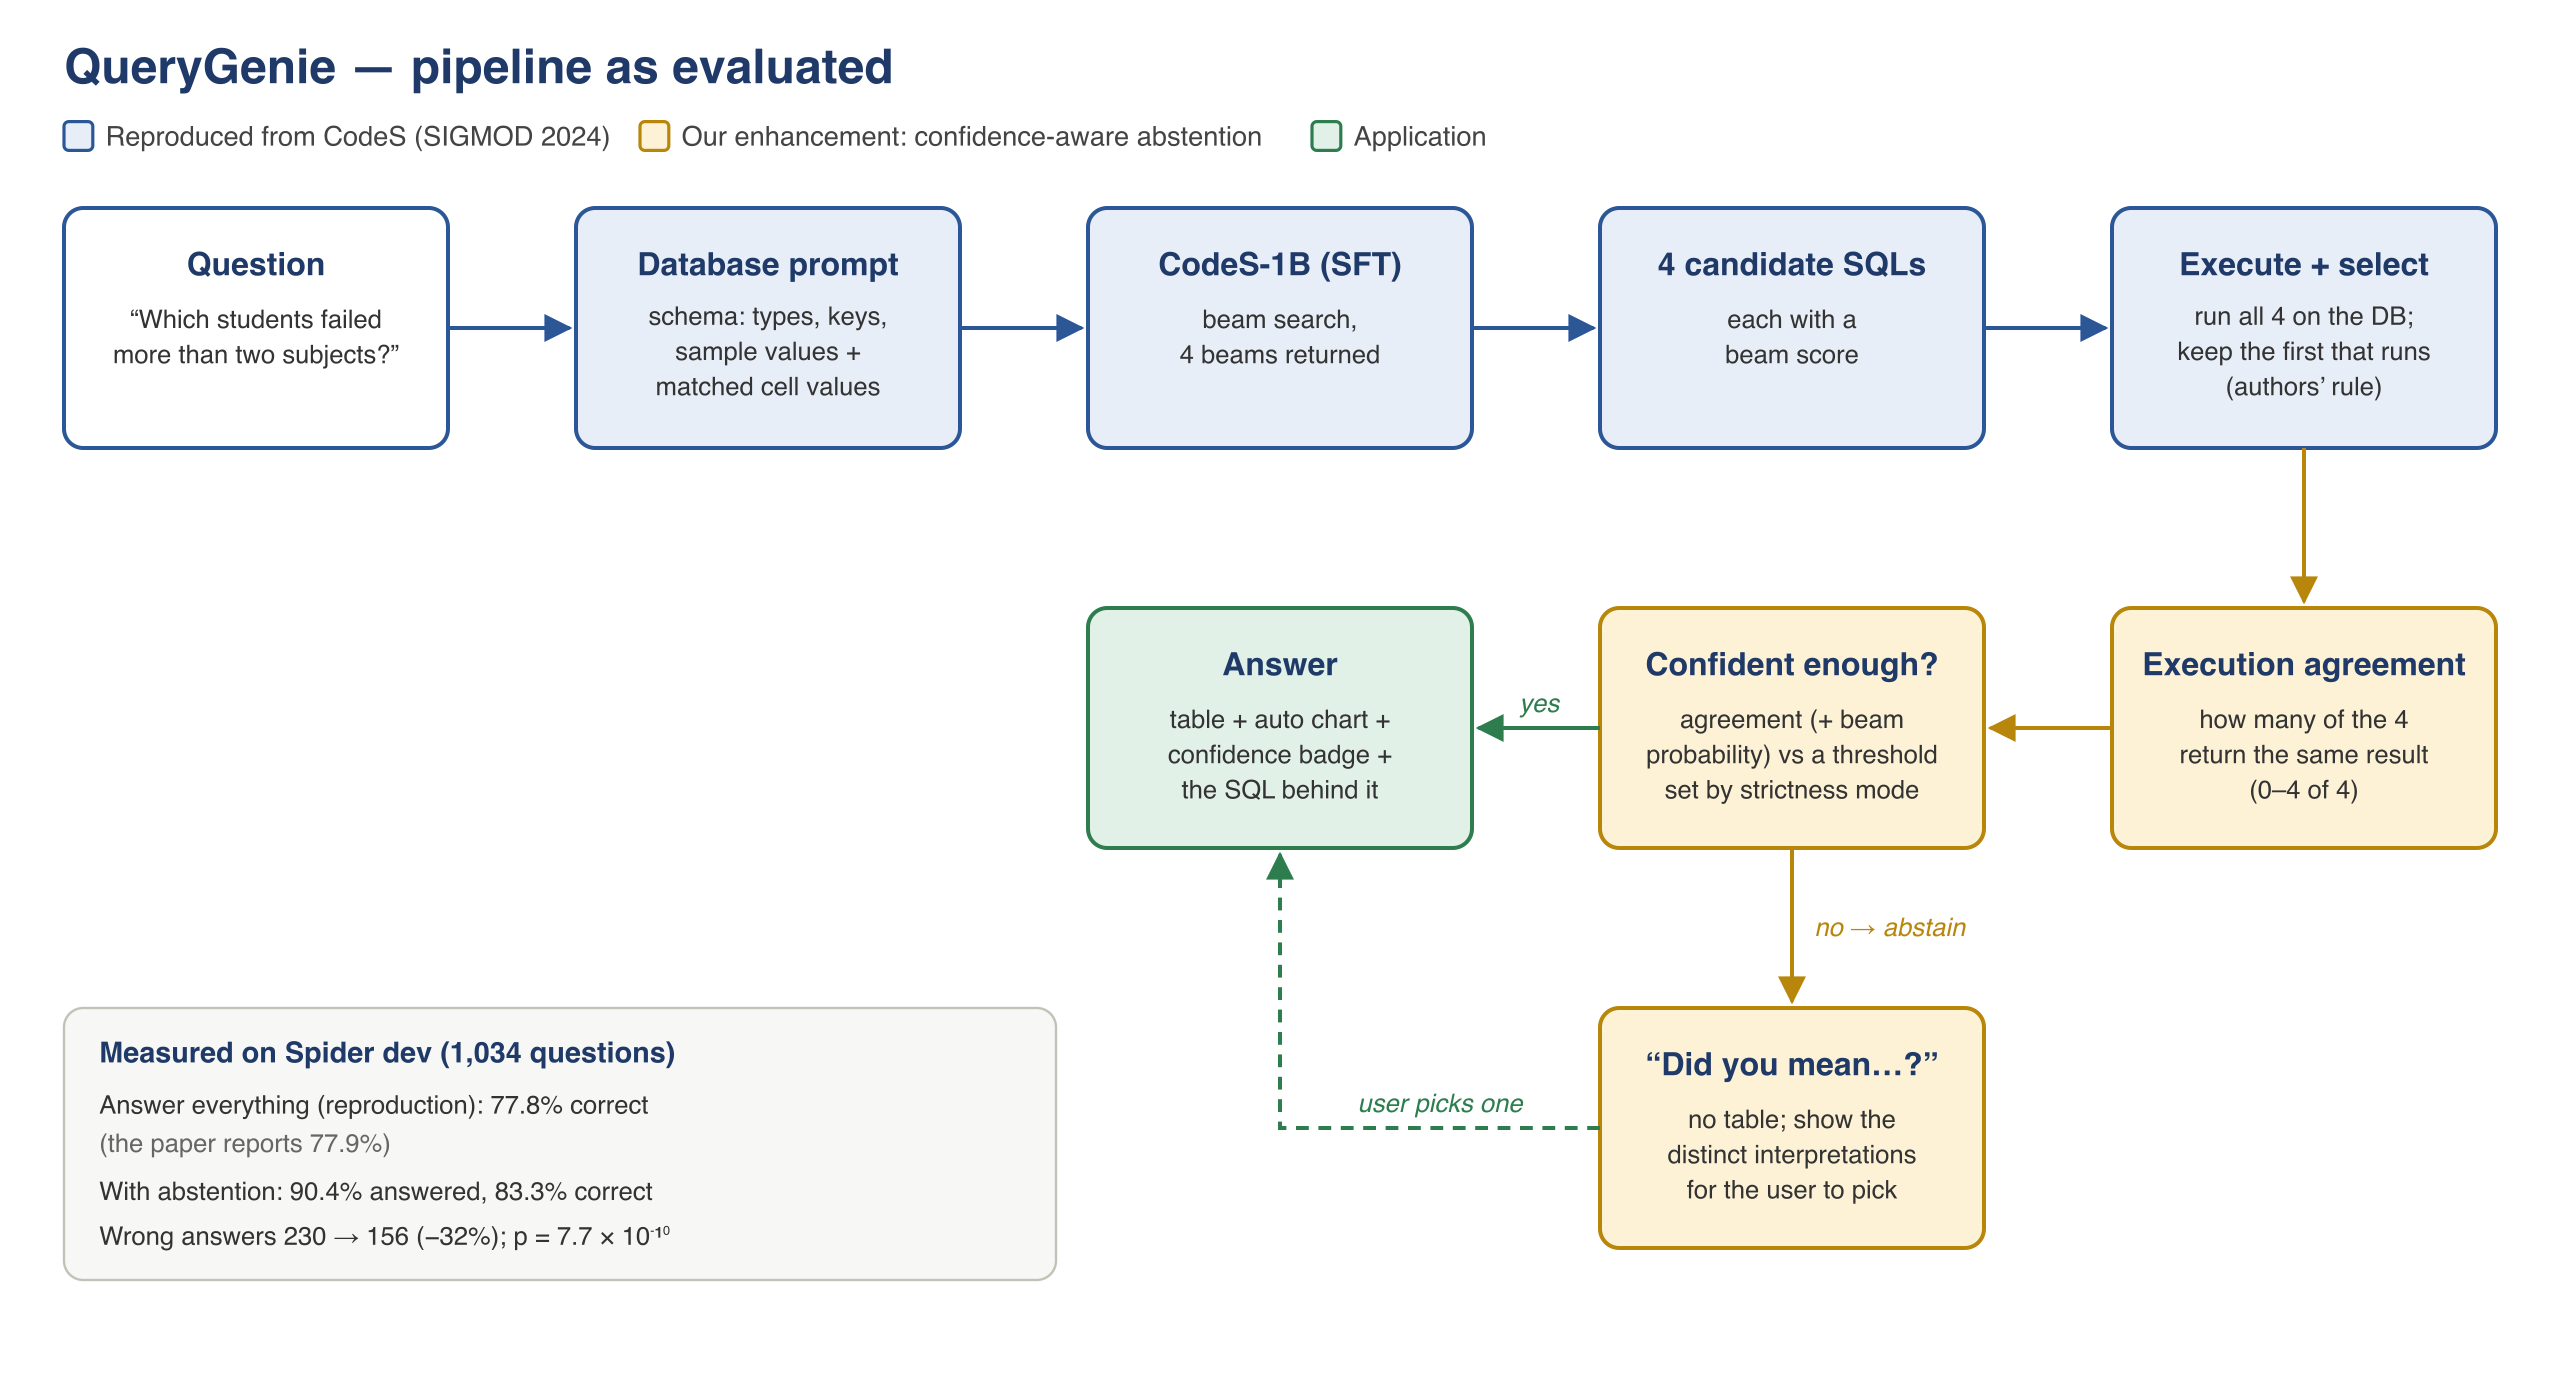
\includegraphics[width=\linewidth]{images/figures/final_pipeline.png}
	\caption{The pipeline as evaluated: reproduced CodeS components (blue), the enhancement (amber) and the application (green).}
	\label{fig:pipeline}
\end{figure}

\section{Reproduction methodology}

\subsection{The CodeS pipeline}

Given a question $Q$ and a database $D$, a text-to-SQL system produces a query $S$ whose result answers $Q$. CodeS builds the database prompt described in Chapter~3 --- schema sequence, column descriptions and the matched cell values --- and appends the question. A schema item classifier can prune the schema to its most relevant tables and columns. The model generates four candidates with beam search, and the first candidate that SQLite accepts is returned. Figure~\ref{fig:codes} summarises the pipeline as annotated from the paper.

\begin{figure}[!t]
	\centering
	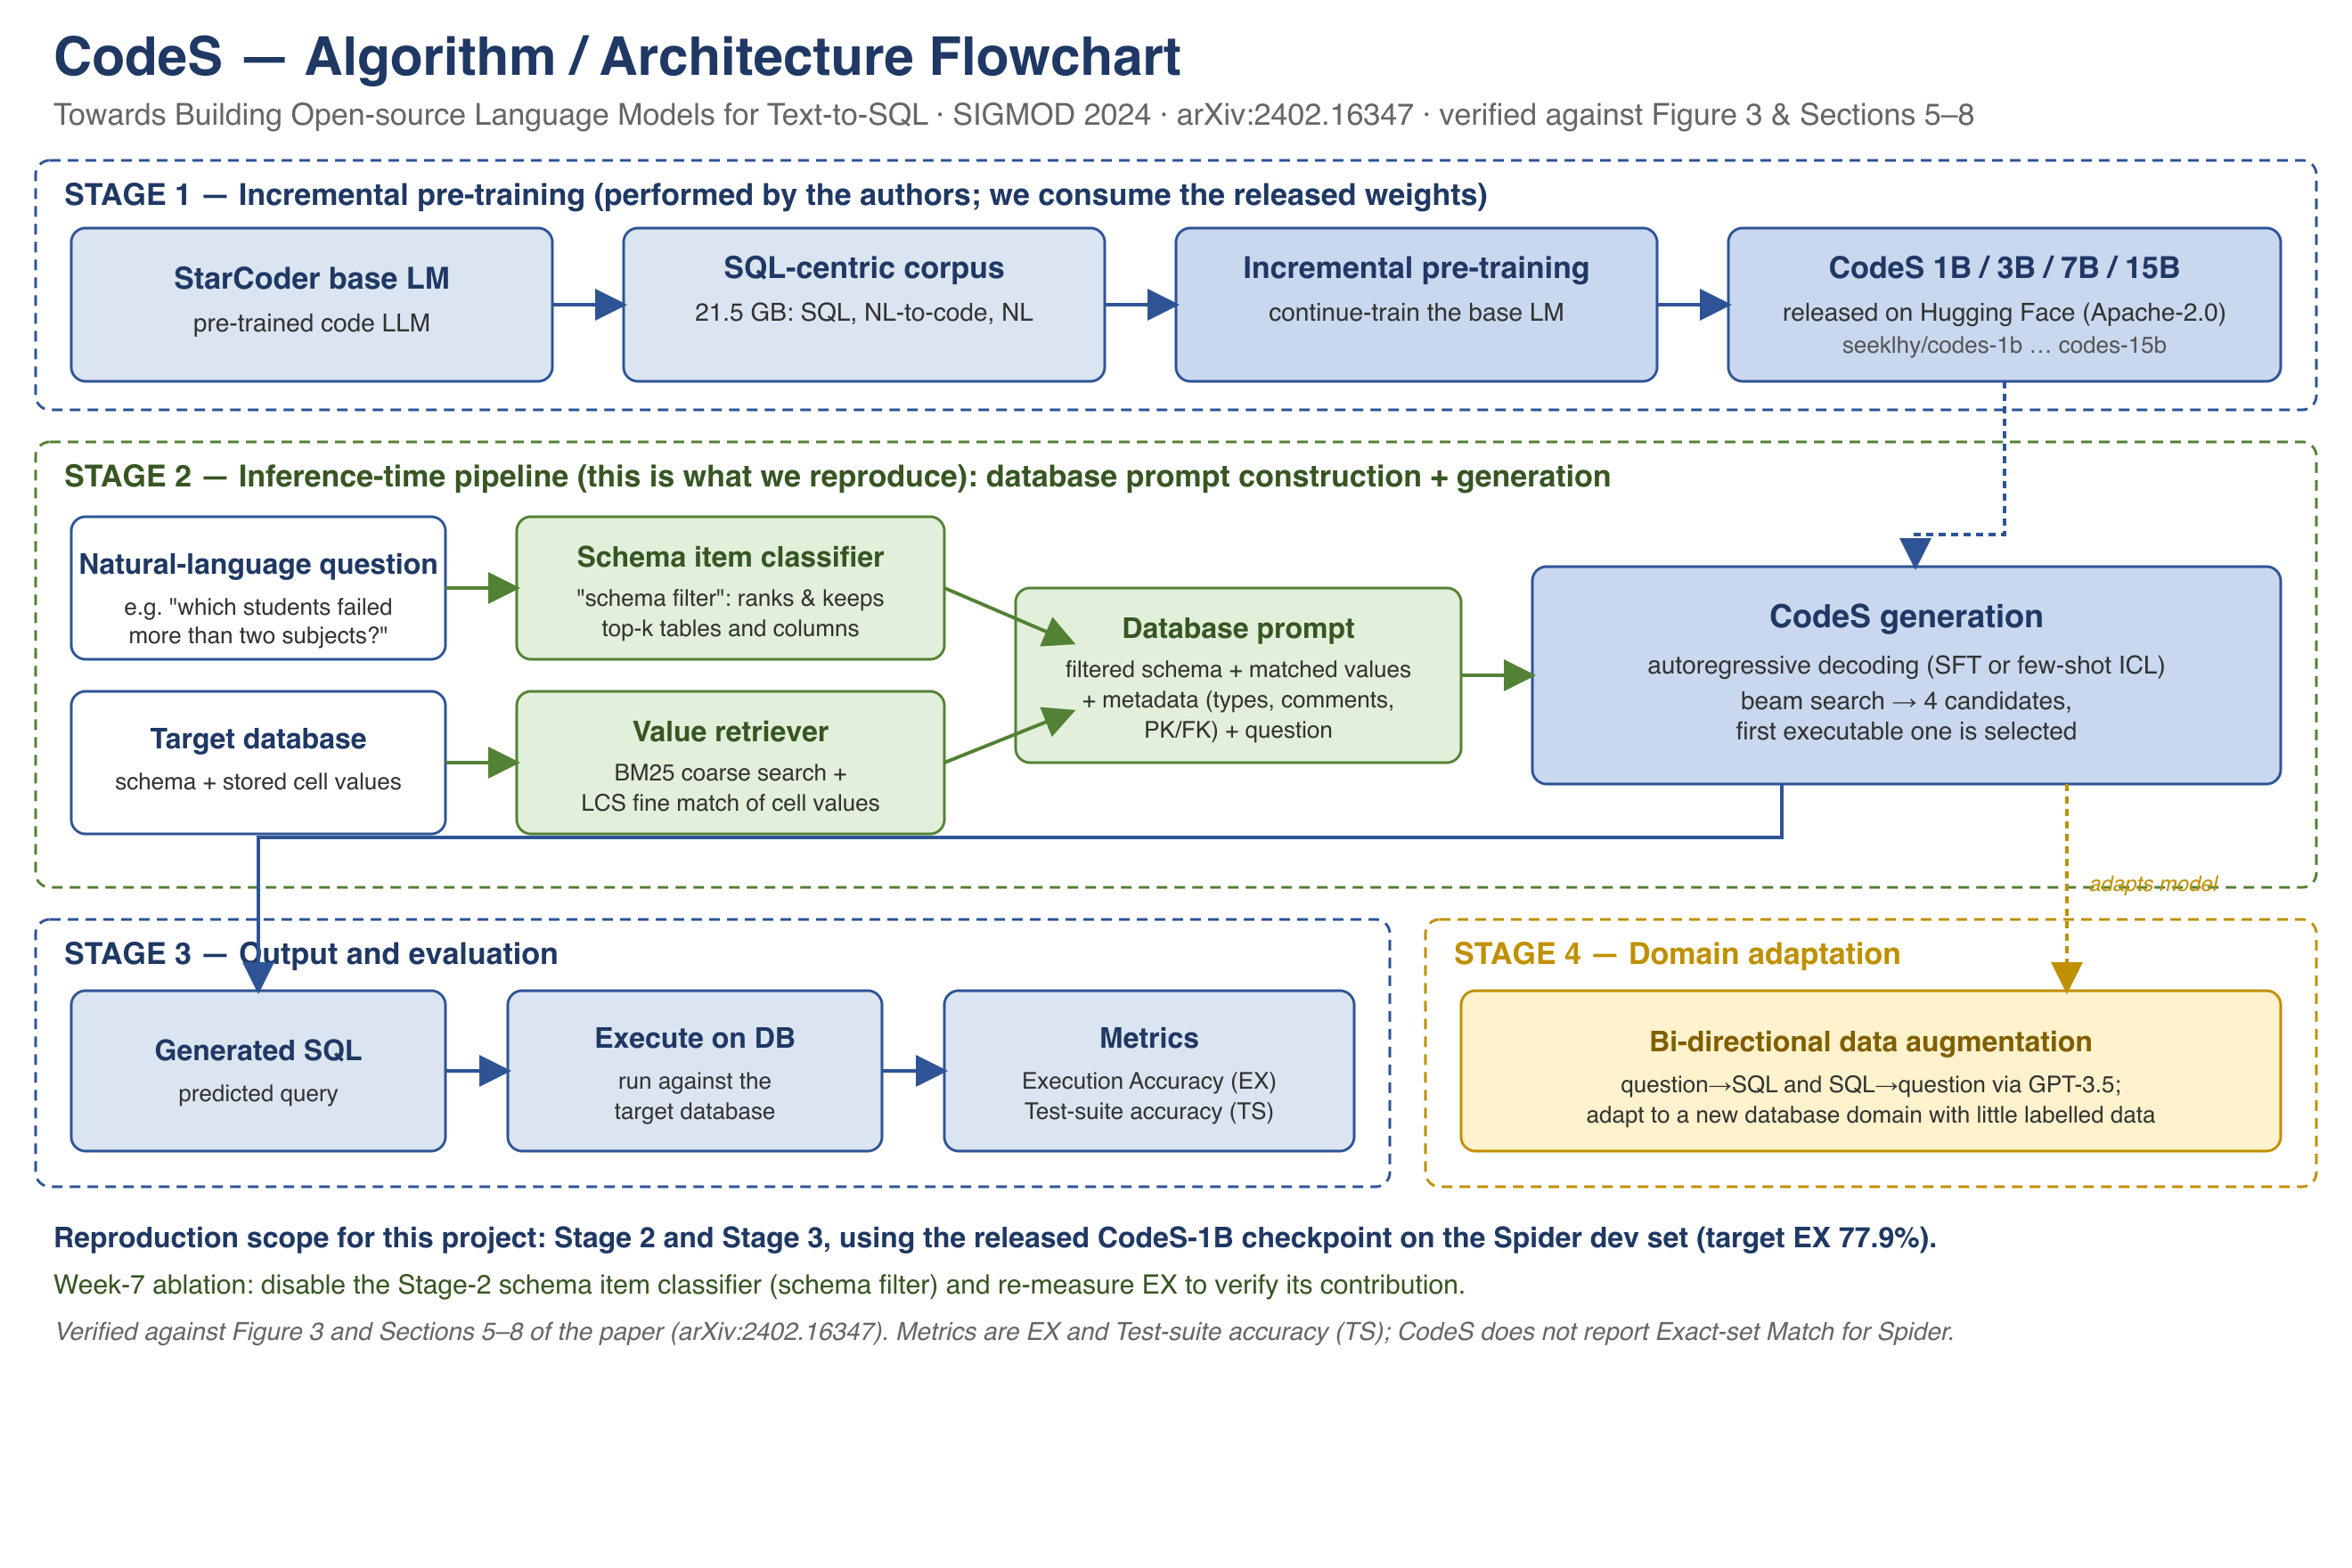
\includegraphics[width=0.92\linewidth]{images/figures/codes_architecture_flowchart.png}
	\caption{The CodeS pipeline, annotated from the paper (Week-3 deliverable).}
	\label{fig:codes}
\end{figure}

\subsection{Environment}

Table~\ref{tab:env} compares the authors' environment with ours. The reproduction first passed the department's Week-4 gate: the released model was loaded on a Colab T4 GPU, generated SQL and executed it against SQLite (run T1-001). The full evaluation followed.

\begin{table}[!t]
	\centering
	\caption{The authors' environment and ours.}
	\label{tab:env}
	\resizebox{\textwidth}{!}{%
	\begin{tabular}{|l|l|l|}
		\hline
		 & \textbf{Authors (official repository)} & \textbf{This project} \\ \hline
		GPU & 8 $\times$ NVIDIA A800, 80\,GB & NVIDIA Tesla T4, 16\,GB (Google Colab); Apple M4, 16\,GB for development \\ \hline
		Precision / batch & fp16, batch size 1 at inference & fp16, batch size 1 \\ \hline
		Python & 3.8.5 & Colab default (3.12.13 at the gate run) \\ \hline
		PyTorch & 1.13.1 & 2.11.0+cu128 \\ \hline
		transformers & 4.28.1 & 5.15.0 (gate run), 5.16.1 (reported runs) \\ \hline
		Dataset & Spider (Google Drive bundle) & Spider from Hugging Face (\path{xlangai/spider}, \path{HAL-9001/spider-databases}) \\ \hline
	\end{tabular}}
\end{table}

\subsection{The reproduced pipeline}

The evaluation harness (\path{research/colab_eval_tier2.py}) reproduces the authors' inference code, and the authors' database utilities are included unmodified (Apache-2.0):

\begin{itemize}
	\item \textbf{Prompt:} schema sequence, matched contents and question, with the beginning-of-sequence token and the authors' left-truncation, exactly as in their \path{prepare_text2sql_prefix_sequence}.
	\item \textbf{Value retriever:} the authors' fine matcher applied to every column's distinct values. The authors first narrow the candidates with a Lucene BM25 index; we scan all values instead (a documented deviation).
	\item \textbf{Decoding and selection:} beam search with four beams, all four returned and post-processed; the first candidate that passes SQLite's \texttt{EXPLAIN QUERY PLAN} is kept, otherwise the first beam --- the rule in the authors' \path{text2sql_zero_shot.py}.
	\item \textbf{Scoring:} the official Spider test-suite evaluator (\texttt{evaluation.py --etype exec}) \cite{zhong2020semantic}, which is what the authors call. Execution Accuracy (EX) counts a prediction as correct when it returns the same result as the gold query; the evaluator treats row order as significant only when the gold query sorts, tolerates reordered columns and ignores \texttt{DISTINCT} by default. Every prediction is saved so that any run can be re-scored.
\end{itemize}

\subsection{Audit of the evaluation harness}

After three runs gave 64.8\%, 71.7\% and 73.8\%, the harness was compared line by line with the authors' code (\path{load_sft_dataset.py}, \path{prepare_sft_datasets.py}, \path{build_contents_index.py}, \path{text2sql_zero_shot.py} and \path{db_utils.py}), and every effect was measured on the full development set. Prompt assembly, decoding, candidate selection and post-processing matched, and the vendored code was identical to the authors'. Four discrepancies were found and fixed:

\begin{enumerate}
	\item \textbf{Value-retriever bug.} The authors index every value as text, numbers included; our port kept only text values, so numbers in questions (``older than 20'') were never matched. This changed the prompt for 128 of the 1,034 questions (12.4\%).
	\item \textbf{Scoring metric.} Our early metric compared sorted rows as strings: it ignored row order and did not accept reordered columns. On the same predictions it gives 73.4\% where the official evaluator gives 77.8\%, so the earlier runs were not on the paper's scale.
	\item \textbf{Column descriptions.} The authors add human-readable column names from Spider's \path{tables.json}; 12 development-set columns are affected.
	\item \textbf{Saved predictions.} Earlier runs did not save their SQL and could not be re-scored.
\end{enumerate}

The official evaluator was checked by scoring the gold queries against themselves (1.000).

\subsection{Run logging and determinism}

Every run is logged with its seed (42), hardware, runtime and library versions in \path{results/reproduction_log.csv} and \path{results/Reproduction_Log.xlsx}, including runs that were later superseded. Beam search is deterministic: repeating a run returned exactly the same predictions (763 of 1,034 correct in T2-003 and its repeat; 759 of 1,034 on the simple metric in T2-005 and T2-006). Differences between runs therefore come from configuration changes, not chance.

\section{Reproducibility results}

\subsection{Run history}

Table~\ref{tab:runs} lists the runs on the development set. The reproduction reached its final figure in steps, and each step isolates a real effect: moving from a schema-only prompt to the authors' full database prompt raised the simple-metric score from 64.8\% to 71.7\%, the authors' candidate-selection rule raised it to 73.8\%, and the audit showed that most of the remaining gap was the scoring metric rather than the model.

\begin{table}[!t]
	\centering
	\caption{Runs on the Spider development set (1,034 questions). ``Simple'' is the early sorted-rows metric; only ``official'' matches the paper.}
	\label{tab:runs}
	\resizebox{\textwidth}{!}{%
	\begin{tabular}{|l|l|l|l|l|}
		\hline
		\textbf{Run} & \textbf{Configuration} & \textbf{Metric} & \textbf{EX} & \textbf{vs 77.9\%} \\ \hline
		T1-001 & Week-4 gate: codes-1b loads, generates and executes SQL (Colab T4) & liveness & passed & --- \\ \hline
		T2-001 & schema and foreign keys only; first beam; Apple M4 & simple & 64.8\% & not comparable \\ \hline
		T2-002 & full CodeS prompt; first beam; Colab T4 & simple & 71.7\% & not comparable \\ \hline
		T2-003 & + authors' candidate selection; Colab T4 (repeated identically) & simple & 73.8\% & not comparable \\ \hline
		T2-005 & audited harness (v2); Colab T4 & official & 77.8\% & $-0.1$ pts \\ \hline
		T2-006 & fresh re-run of T2-005 (Week-10 baseline) & official & 77.76\% (804/1,034) & $-0.14$ pts \\ \hline
	\end{tabular}}
\end{table}

\subsection{Headline comparison}

Scored with the paper's own evaluator, the reproduced CodeS-1B reaches \textbf{77.8\% Execution Accuracy against the reported 77.9\%}: a difference of 0.1 points, well inside the department's tolerance. The fresh Week-10 re-run gave the identical result (804 of 1,034 correct). 97.3\% of the predictions execute.

Test-suite accuracy (paper: 72.2\%) requires the distilled test-suite databases, which are distributed on Google Drive and were not obtained; our test-suite accuracy is \textbf{TBD}. The saved predictions of T2-006 can be scored for it without re-running the model.

\subsection{Ablation study}

Each component of the pipeline was disabled in turn and the full development set re-evaluated with the official evaluator (runs AB-103 to AB-106, Colab T4). Table~\ref{tab:ablation} and Figure~\ref{fig:ablation} give the results.

\begin{table}[!t]
	\centering
	\caption{Ablation study, official evaluator.}
	\label{tab:ablation}
	\begin{tabular}{|l|r|r|r|}
		\hline
		\textbf{Component removed} & \textbf{EX} & \textbf{Change} & \textbf{Executable} \\ \hline
		--- (full pipeline, T2-005) & 77.8\% & --- & 97.3\% \\ \hline
		Foreign-keys block & 76.9\% & $-0.9$ & 95.9\% \\ \hline
		Representative column values & 76.4\% & $-1.4$ & 98.1\% \\ \hline
		Candidate selection (first beam only) & 76.0\% & $-1.8$ & 94.1\% \\ \hline
		Value retriever (matched contents) & 75.9\% & $-1.9$ & 97.2\% \\ \hline
	\end{tabular}
\end{table}

\begin{figure}[!t]
	\centering
	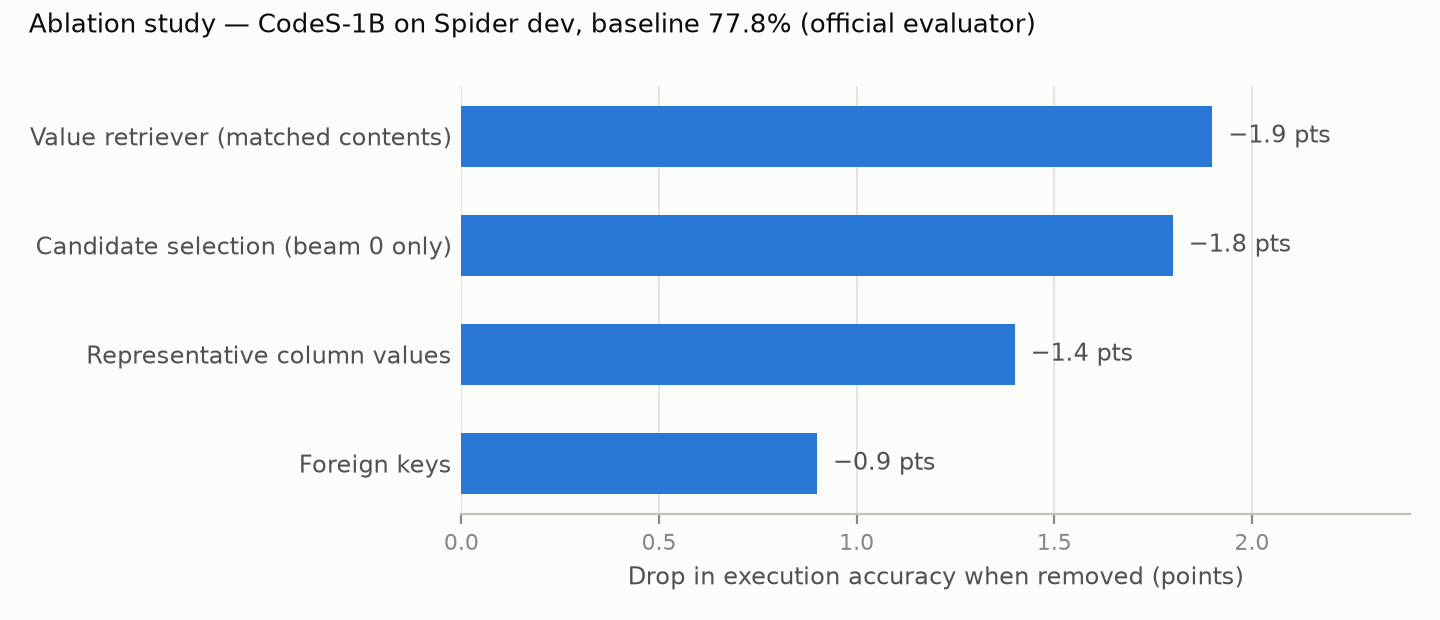
\includegraphics[width=0.8\linewidth]{images/figures/ablation_official.png}
	\caption{Drop in Execution Accuracy when each component is removed.}
	\label{fig:ablation}
\end{figure}

Every component contributes. The value retriever matters most, and the way it matters is telling: without it almost as many queries still execute (97.2\%) --- the model writes runnable SQL with the wrong literal values, so the answers are silently wrong. Candidate selection works differently: it is the ablation that reduces executability most (94.1\%), because it is what replaces a broken first beam with a working alternative. Without the foreign keys the model guesses join conditions, which also shows up as lower executability. These differences are 9 to 20 questions each and were not tested for significance individually.

\section{Enhancement: confidence-aware abstention}

\subsection{Choice and justification}

The department allows one enhancement, chosen from defined tiers and approved by the guide. The Week-1 abstract had named execution-guided self-correction, the strategy of DIN-SQL \cite{pourreza2023dinsql}. The reproduction showed that 97.3\% of predictions already execute, so repairing failed queries could recover at most 2.7 points and was unlikely to produce a significant gain. The ablation and the difficulty analysis of Chapter~3 showed instead that the dominant error is a query that runs but returns the wrong rows. We therefore proposed confidence-aware abstention (Tier 4, a novel combination), keeping self-correction and automatic charts as application features.

That expectation was later measured directly (\path{research/repair_eval.py}). Keeping the four candidates of run T2-006 fixed, every failed candidate --- 377 queries in 211 questions --- was sent back to CodeS-1B once with its database error. Only 61 of the repaired queries ran, and one answer became correct (none became wrong): Execution Accuracy moved from 77.76\% to 77.85\%, and the tested abstention setting from 90.43\% coverage at 83.32\% to 90.52\% at 83.23\%. CodeS was fine-tuned on question--SQL pairs and never learned to use error feedback, which DIN-SQL's self-correction relies on. Self-correction therefore remains an application feature, on by default and labelled as such, and is not part of the evaluated results.

\subsection{Method}

The pipeline already produces four beam candidates per question. All four are executed. The confidence of the returned answer is the share of candidates whose result equals it --- execution agreement, from 0 to 4 of 4, and zero when the returned query does not run --- with the beam probability of the returned candidate (the softmax of the four beam scores) used only to break ties. The idea combines self-consistency \cite{wang2022selfconsistency} with selective classification \cite{geifman2017selective}. When confidence is below a threshold the system abstains: it shows no table and offers the distinct results of the candidates as interpretations for the user to choose from. No retraining is involved. Algorithm~\ref{alg:abstain} states the procedure.

\begin{algorithm}[!t]
	\SetAlgoLined
	\KwIn{question $Q$, database $D$, threshold $\tau$}
	\KwOut{an answer, or the readings for the user to choose from}
	$P \leftarrow$ CodeS database prompt for $(Q, D)$\;
	$(s_1, \dots, s_4), (b_1, \dots, b_4) \leftarrow$ four beam candidates and their scores\;
	\For{$i \leftarrow 1$ \KwTo $4$}{
		$r_i \leftarrow$ result of executing $s_i$ on $D$ (read-only; empty if it fails)\;
	}
	$k \leftarrow$ first $i$ whose query passes \texttt{EXPLAIN QUERY PLAN}, else $1$\;
	$a \leftarrow \frac{1}{4}\,\lvert\{\, i : r_i = r_k \,\}\rvert$ if $s_k$ runs, else $0$\;
	$p \leftarrow e^{b_k} / \sum_j e^{b_j}$\;
	$c \leftarrow a + 0.01\,p$\;
	\eIf{$c \ge \tau$}{
		\Return result $r_k$ with confidence $a$\;
	}{
		\Return the distinct results among $r_1, \dots, r_4$ as readings\;
	}
	\caption{Confidence-aware abstention on top of CodeS}
	\label{alg:abstain}
\end{algorithm}

\subsection{Hypothesis and protocol}

The hypothesis and protocol were fixed before the results were seen.

\begin{itemize}
	\item \textbf{H1:} at the same coverage, accuracy on answered questions is higher with agreement-based abstention than with random abstention, and higher than the 77.8\% baseline. \textbf{H0:} no difference.
	\item \textbf{Protocol:} 10 random 50/50 splits of the development set. On the calibration half the threshold is set for at least 90\% coverage, then applied to the test half. The paired quantity is the accuracy on answered test questions minus the expected accuracy of random abstention at the same coverage, which is the test half's full-coverage accuracy. One-sided paired t-test and Wilcoxon signed-rank test, $\alpha = 0.05$.
	\item \textbf{Data:} one run (T2-006) recording, for every question, all four candidates with their beam scores, execution results and official correctness, checked to add up to the evaluator's total. The original and the enhanced systems are therefore compared on exactly the same predictions.
\end{itemize}

The threshold used by the application, $\tau = 0.2526$, is the median of the 10 calibration-half thresholds. In words: abstain when no candidate executes, or when only 1 of 4 candidates supports the answer and its beam probability is below about 0.26.

\subsection{Results}

Table~\ref{tab:enh} compares the original and enhanced systems on the same 1,034 questions, and Table~\ref{tab:sig} gives the significance tests.

\begin{table}[!t]
	\centering
	\caption{Original against enhanced on the same 1,034 questions.}
	\label{tab:enh}
	\resizebox{\textwidth}{!}{%
	\begin{tabular}{|l|r|r|r|}
		\hline
		\textbf{System} & \textbf{Answered} & \textbf{Accuracy on answered} & \textbf{Wrong answers} \\ \hline
		CodeS-1B, paper (Table 5) & 1,034 (100\%) & 77.9\% & --- \\ \hline
		Original --- CodeS-1B reproduced & 1,034 (100\%) & 77.76\% & 230 \\ \hline
		Enhanced --- tested setting & 935 (90.4\%) & 83.32\% & 156 \\ \hline
		Enhanced --- 3 of 4 agree & 649 (62.8\%) & 86.13\% & 90 \\ \hline
		Enhanced --- all 4 agree & 412 (39.8\%) & 88.35\% & 48 \\ \hline
	\end{tabular}}
\end{table}

\begin{table}[!t]
	\centering
	\caption{Significance tests over 10 calibration/test splits (mean coverage 90.5\%) and a 5,000-sample bootstrap over questions.}
	\label{tab:sig}
	\resizebox{\textwidth}{!}{%
	\begin{tabular}{|l|l|l|l|l|}
		\hline
		\textbf{Signal} & \textbf{Mean gain} & \textbf{Paired t-test (df 9)} & \textbf{Wilcoxon} & \textbf{Bootstrap 95\% CI} \\ \hline
		Execution agreement & $+5.46$ pts (SD 0.71) & $t = 24.44$, $p = 7.7 \times 10^{-10}$ & $W = 55$, $p = 9.8 \times 10^{-4}$ & $[+4.51, +6.71]$ \\ \hline
		Beam probability (comparison) & $+3.08$ pts (SD 0.90) & $t = 10.81$, $p = 9.3 \times 10^{-7}$ & $W = 55$, $p = 9.8 \times 10^{-4}$ & $[+1.97, +3.94]$ \\ \hline
	\end{tabular}}
\end{table}

H0 is rejected. All 10 splits showed a positive gain ($W = 55$ is the maximum, and $9.8 \times 10^{-4}$ the smallest p-value the Wilcoxon test can give with 10 pairs). Because the splits reuse the same questions, the questions themselves were also resampled 5,000 times; no resample showed a gain of zero or less. At the tested setting the system declines 99 questions, 74 of which it would have answered wrongly and 25 correctly: wrong answers fall by 32\% at the cost of withholding 3.1\% of the correct ones.

Figure~\ref{fig:coverage} shows the whole accuracy--coverage curve, and Table~\ref{tab:calib} shows that the signal is calibrated: accuracy rises steadily with agreement.

\begin{figure}[!t]
	\centering
	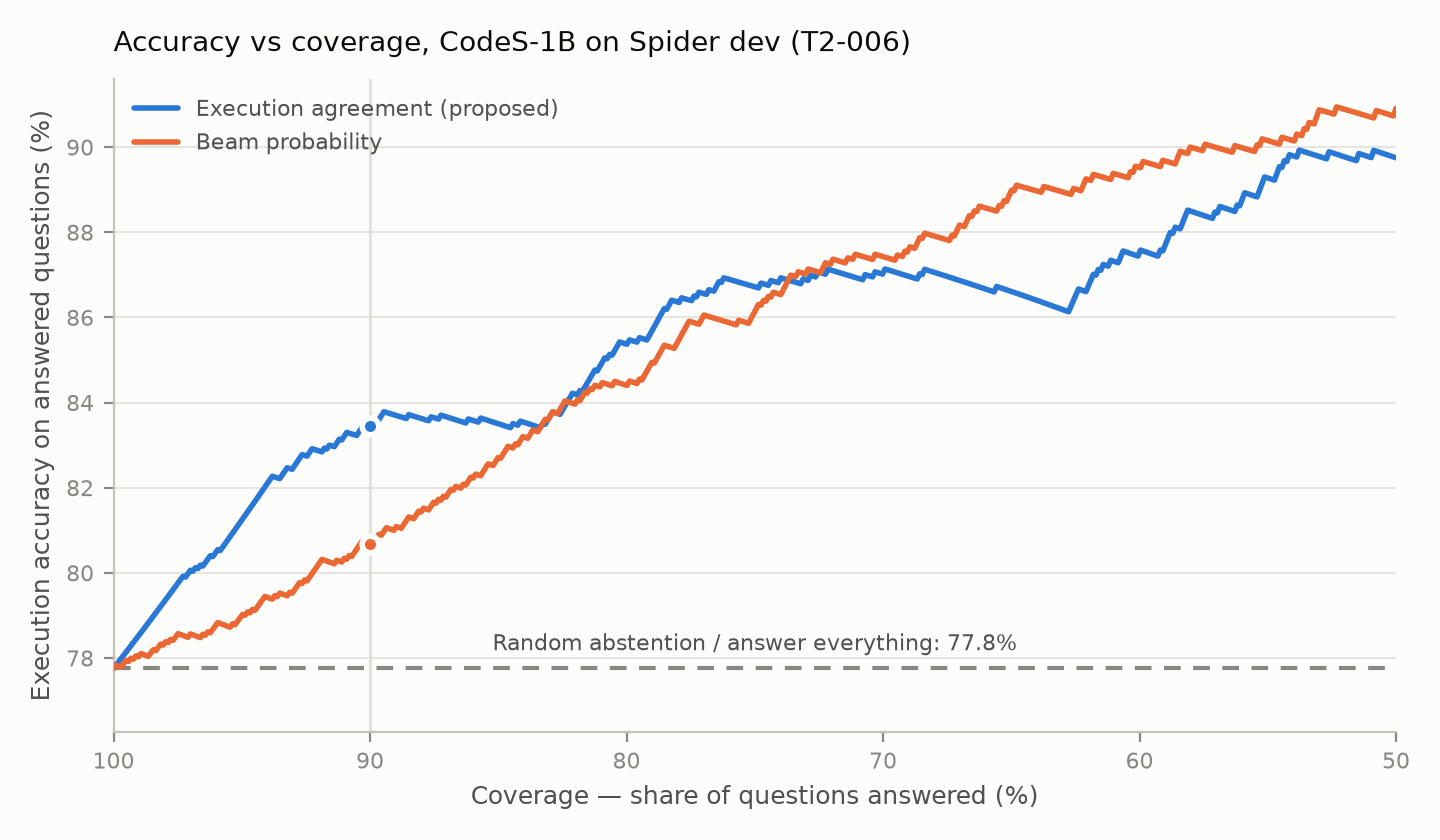
\includegraphics[width=0.8\linewidth]{images/figures/accuracy_coverage_T2-006.png}
	\caption{Accuracy on answered questions against coverage. The dashed line is the original system (and random abstention); dots mark 90\% coverage.}
	\label{fig:coverage}
\end{figure}

\begin{table}[!t]
	\centering
	\caption{Accuracy by the number of candidates agreeing with the answer.}
	\label{tab:calib}
	\begin{tabular}{|l|r|r|}
		\hline
		\textbf{Candidates agreeing with the answer} & \textbf{Questions} & \textbf{Accuracy} \\ \hline
		None (selected query does not run) & 28 & 0.0\% \\ \hline
		1 of 4 & 132 & 56.8\% \\ \hline
		2 of 4 & 225 & 75.6\% \\ \hline
		3 of 4 & 237 & 82.3\% \\ \hline
		4 of 4 & 412 & 88.3\% \\ \hline
	\end{tabular}
\end{table}

\subsection{Agreement for choosing, not only for abstaining?}

A natural question is whether agreement could also raise plain Execution Accuracy, by returning the answer most candidates agree on instead of the first one that executes. Table~\ref{tab:select} answers it from the same four-candidate record (\path{research/selection_analysis.py}; no model run). Majority vote is \emph{worse}: it changes the selection on 69 questions, 11 of which become correct and 32 wrong, so accuracy falls from 77.76\% to 75.73\%. When the candidates split, the first beam is right more often than the majority. Agreement is therefore a good signal for deciding \emph{whether} to trust an answer, which is how the enhancement uses it, but not for deciding \emph{which} answer to give.

\begin{table}[!t]
	\centering
	\caption{Choosing among the four candidates of run T2-006.}
	\label{tab:select}
	\begin{tabular}{|l|r|r|}
		\hline
		\textbf{Selection rule} & \textbf{Correct} & \textbf{EX} \\ \hline
		First candidate that executes (CodeS, reproduced) & 804 & 77.76\% \\ \hline
		Majority vote over the candidates' results & 783 & 75.73\% \\ \hline
		Upper bound: a correct candidate is among the four & 859 & 83.08\% \\ \hline
	\end{tabular}
\end{table}

The upper bound shows the room that remains: a correct query is among the four candidates for 83.1\% of questions, while the selection rule picks it for 77.8\%. Closing part of that gap would need a learned reranker, which is left as future work.

\subsection{Limits of the enhancement}

\begin{itemize}
	\item \textbf{Beam probability is the better signal when abstaining heavily.} Execution agreement is ahead from 100\% down to about 74\% coverage --- the region where a usable assistant operates and where the proposal set its operating point --- but below 74\% beam probability is ahead, and over the whole curve it has the lower area under the risk--coverage curve (0.091 against 0.103; random 0.222, perfect ranking 0.027).
	\item \textbf{Agreement is not proof.} 11.7\% of the answers on which all four candidates agree are still wrong; abstention reduces errors but does not remove them.
	\item \textbf{One model, one benchmark.} The threshold was calibrated on Spider with CodeS-1B; its behaviour with other models, and on real institutional databases, is not measured.
	\item \textbf{Statistical independence.} The 10 splits reuse the same questions, so their p-values are optimistic; the question-level bootstrap is the check that does not depend on this.
\end{itemize}

\section{The application}

The enhancement is delivered in QueryGenie, a desktop application for macOS and Windows, which meets the department's requirement for a full-stack deliverable rather than a notebook. On first start a setup assistant checks the computer and downloads the model (\path{seeklhy/codes-1b-spider}, about 4.5\,GB) and, optionally, the 20 Spider development databases. It then runs exactly the evaluated pipeline, locally.

\begin{itemize}
	\item \textbf{Chats.} Questions are asked in chats, one database at a time. Every answer shows how many of the four candidate queries agree (Figure~\ref{fig:app-answer}), the results table, an automatically chosen chart, the SQL behind the table (editable, and re-runnable read-only) and all four candidates.
	\item \textbf{Abstention.} When the candidates disagree beyond the chosen strictness setting, the application withholds the table and shows the distinct readings for the user to choose from (Figure~\ref{fig:app-notsure}). The four strictness settings display their measured coverage and accuracy from Table~\ref{tab:enh}.
	\item \textbf{Schema map.} The whole database is drawn as a tree of tables, columns, keys and links; tapping a table or column offers questions about it (Figure~\ref{fig:app-map}).
	\item \textbf{Databases.} Besides the sample and Spider databases, users can open their own SQLite files or connect to PostgreSQL and MySQL servers. Every query is checked to be a single read-only statement and runs inside a read-only transaction with a timeout and a row limit. The model writes SQLite-style SQL, which is translated to the server's dialect: on the Spider databases loaded into PostgreSQL, translated queries return the same answer as on SQLite for 94.4\% of gold queries and 93.7\% of the model's predictions. Accuracy and confidence were calibrated on SQLite only.
	\item \textbf{Other models.} The evaluated CodeS-1B model is the default. The user can also choose the earlier prototype's CodeS variants, any model run by Ollama, an OpenAI-compatible server, or cloud services (Figure~\ref{fig:app-picker}). They receive the same four-candidate confidence check, but their accuracy was not measured, and the application labels their confidence as not calibrated. Cloud services receive the schema, a few example values and the question, never result rows, and only after the user confirms.
\end{itemize}

By default everything runs on the user's computer on open weights, so no schema or data leaves the machine.

\begin{figure}[!t]
	\centering
	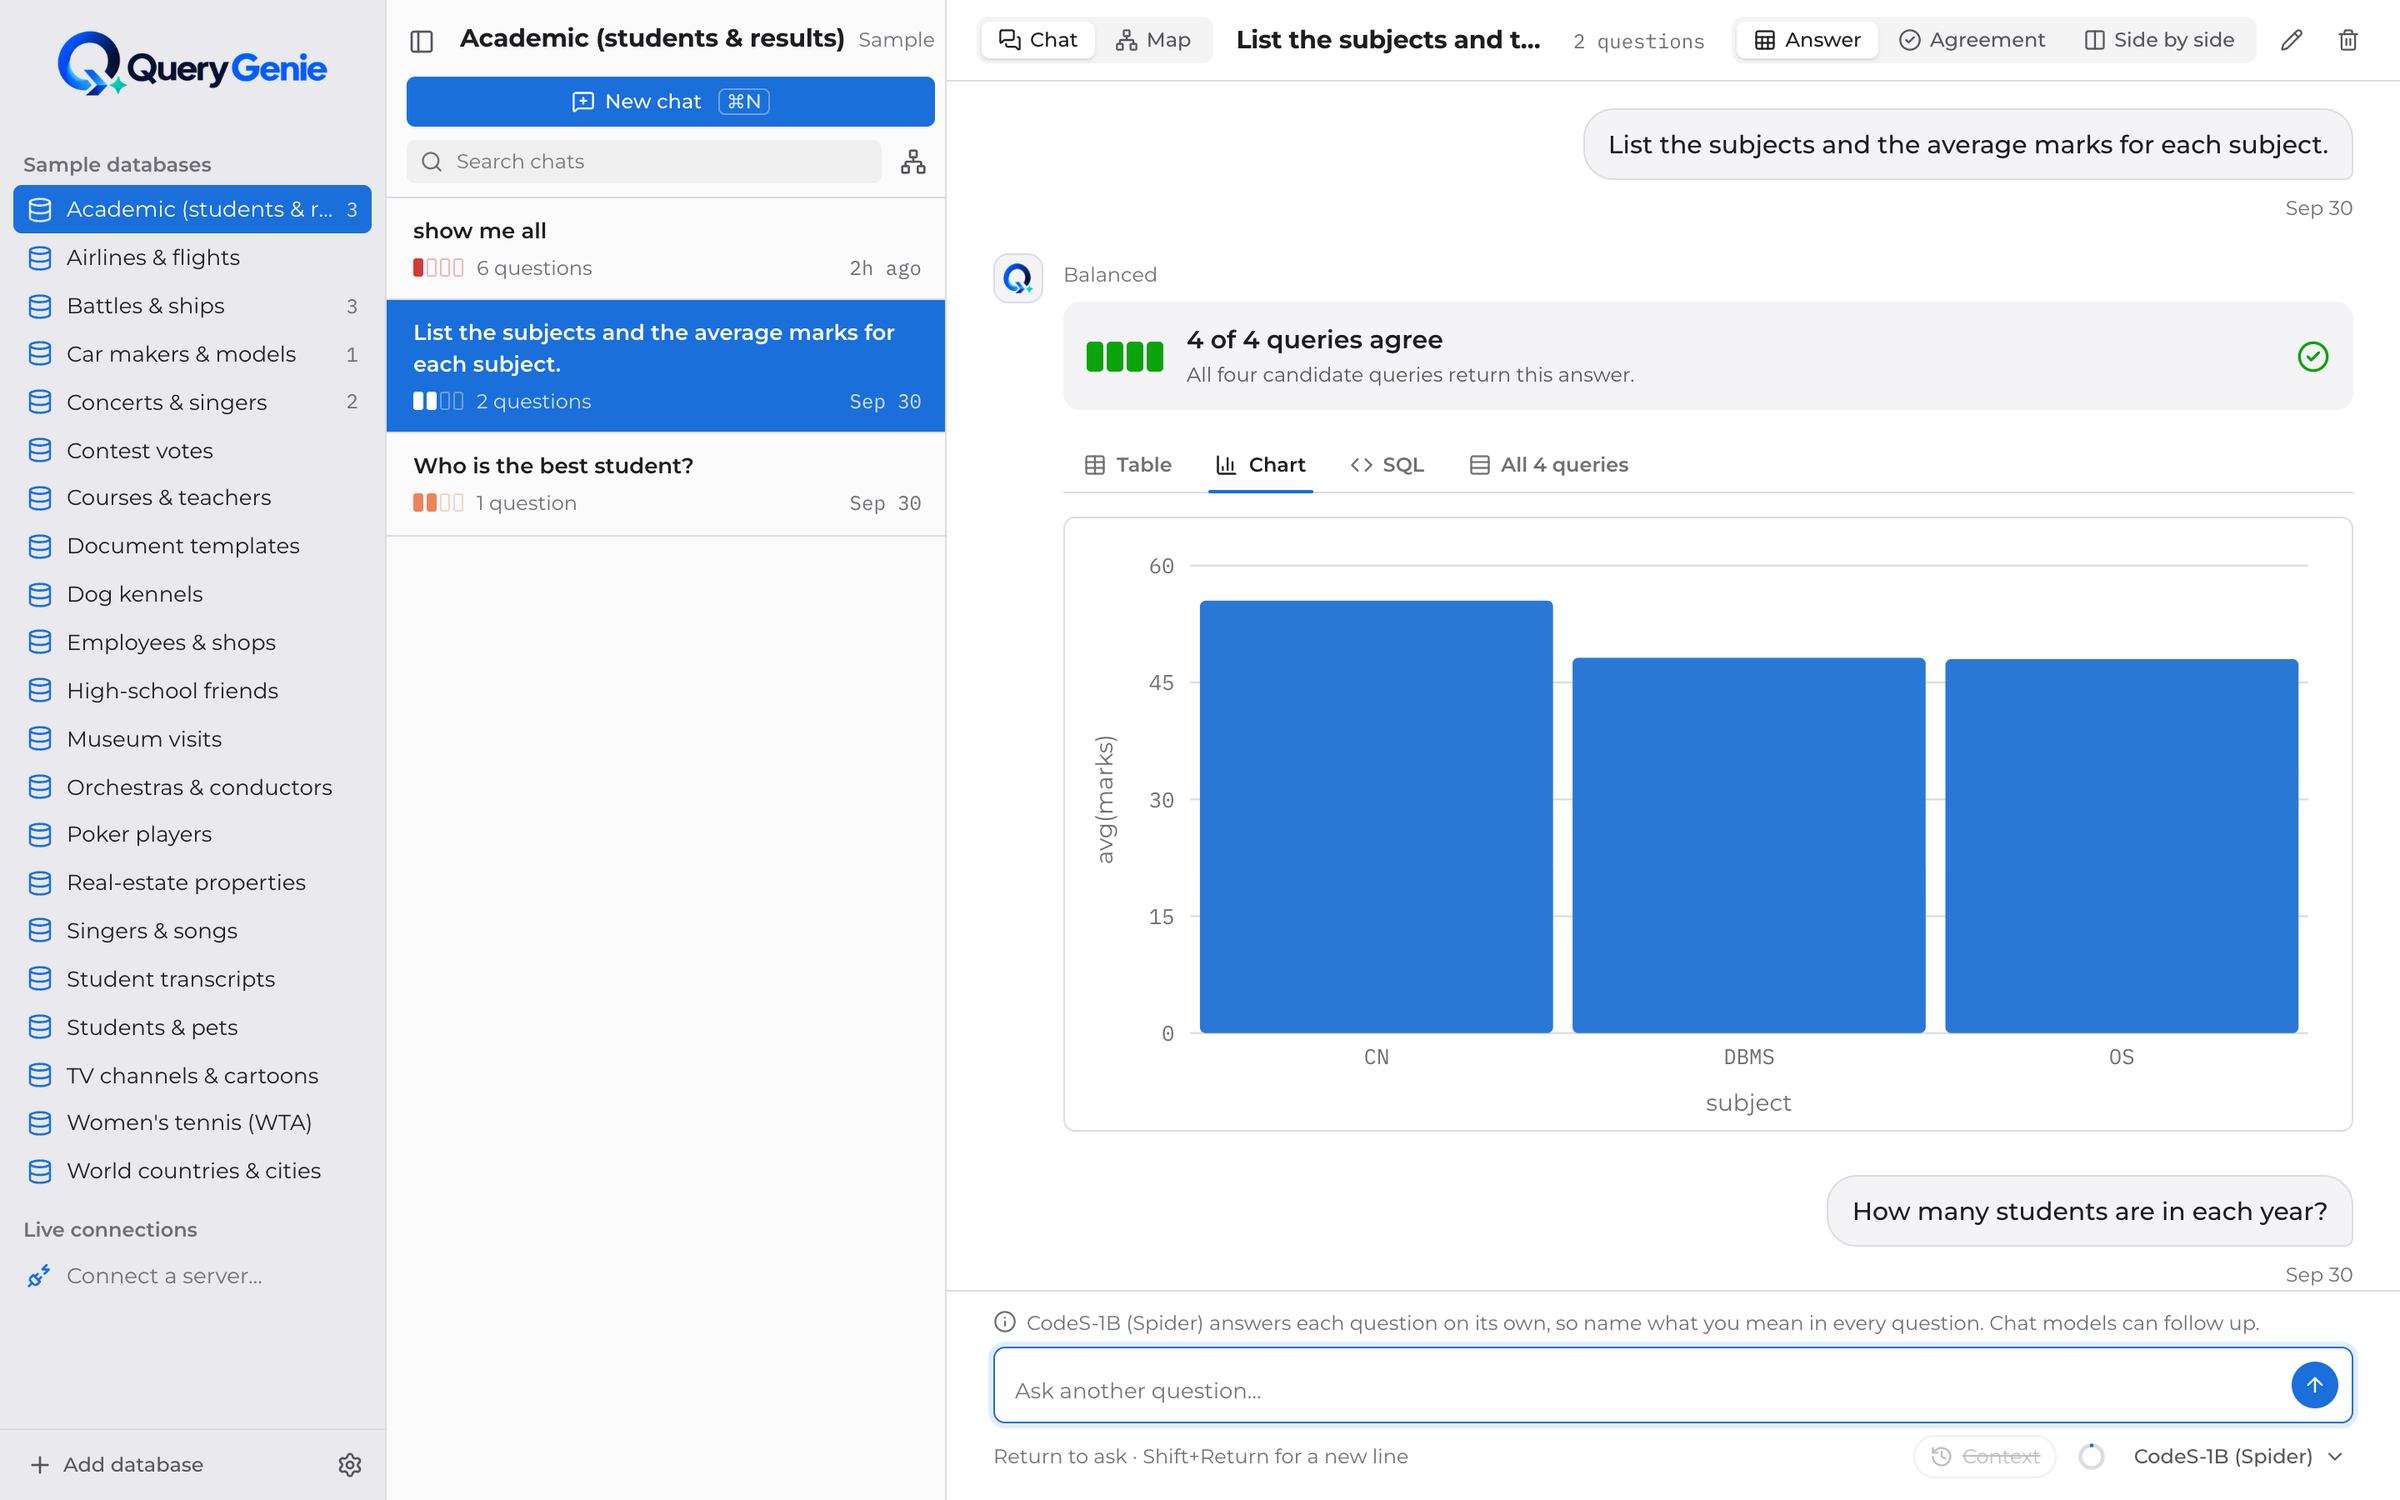
\includegraphics[width=\linewidth]{images/figures/app_answer.png}
	\caption{An answer with its confidence: two of the four candidate queries agree, so the answer is shown as low confidence, with the other reading offered.}
	\label{fig:app-answer}
\end{figure}

\begin{figure}[!t]
	\centering
	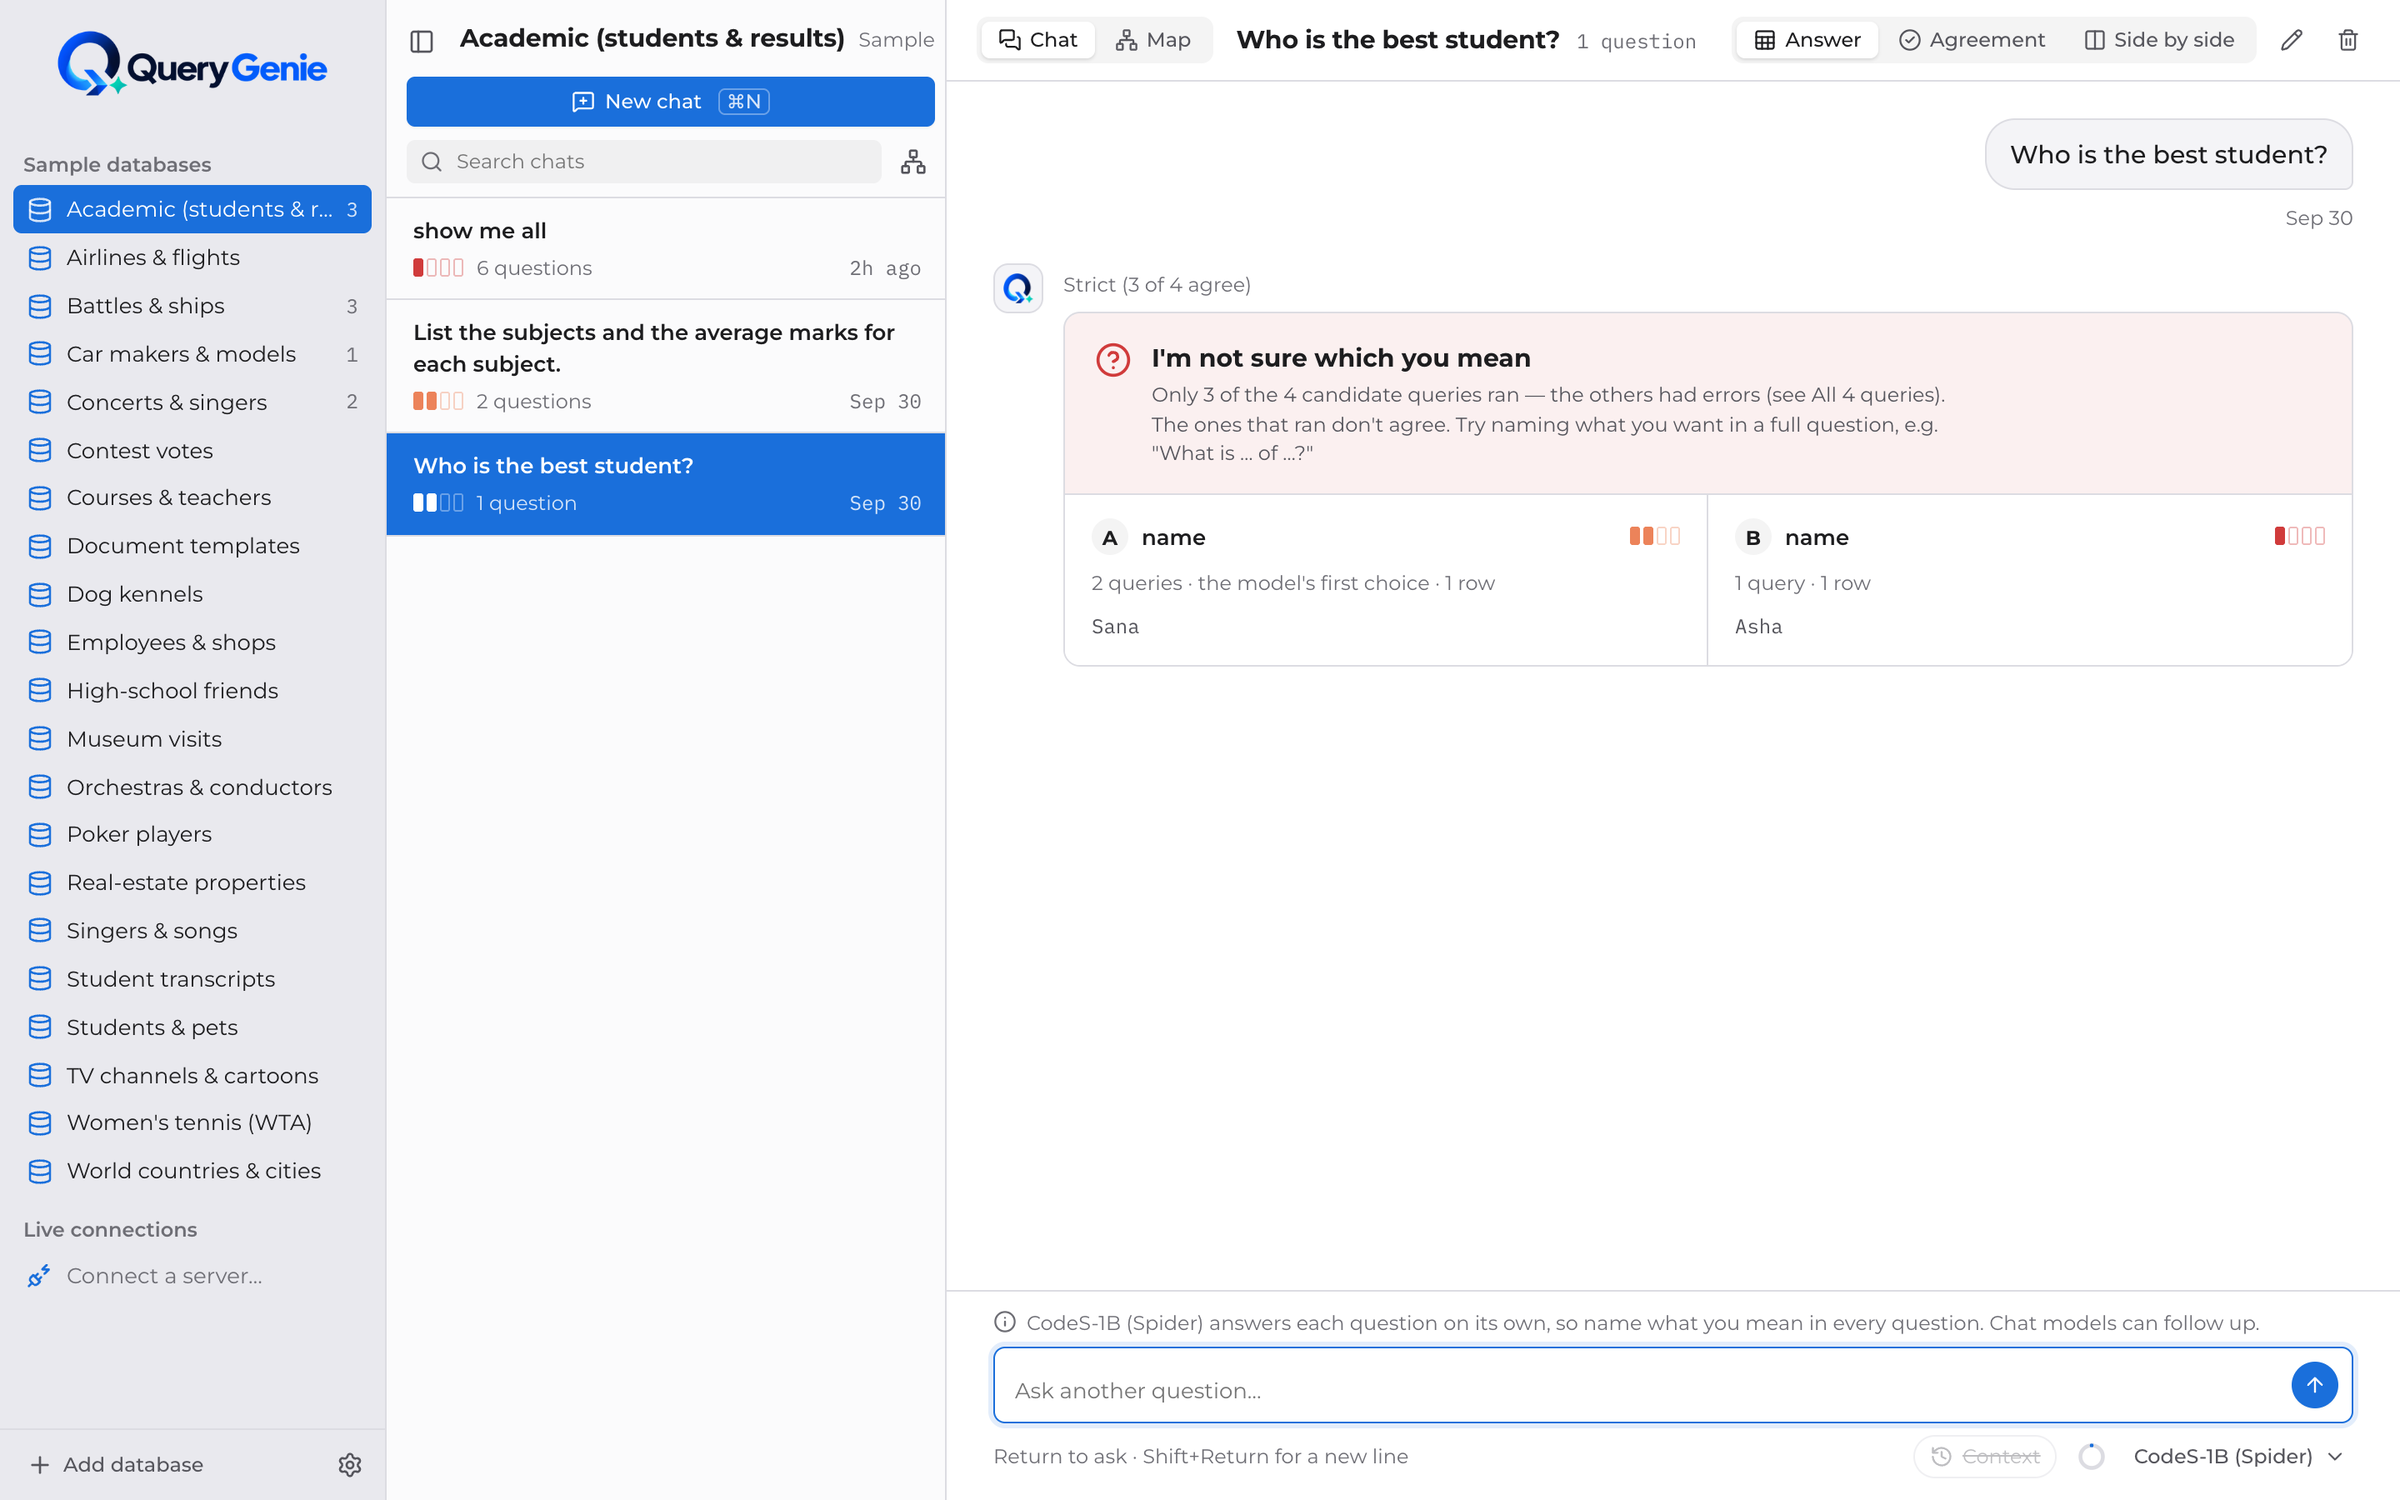
\includegraphics[width=\linewidth]{images/figures/app_not_sure.png}
	\caption{Abstention under the strict setting: the candidates split two against two on the flagship question, so the application asks which reading was meant instead of guessing.}
	\label{fig:app-notsure}
\end{figure}

\begin{figure}[!t]
	\centering
	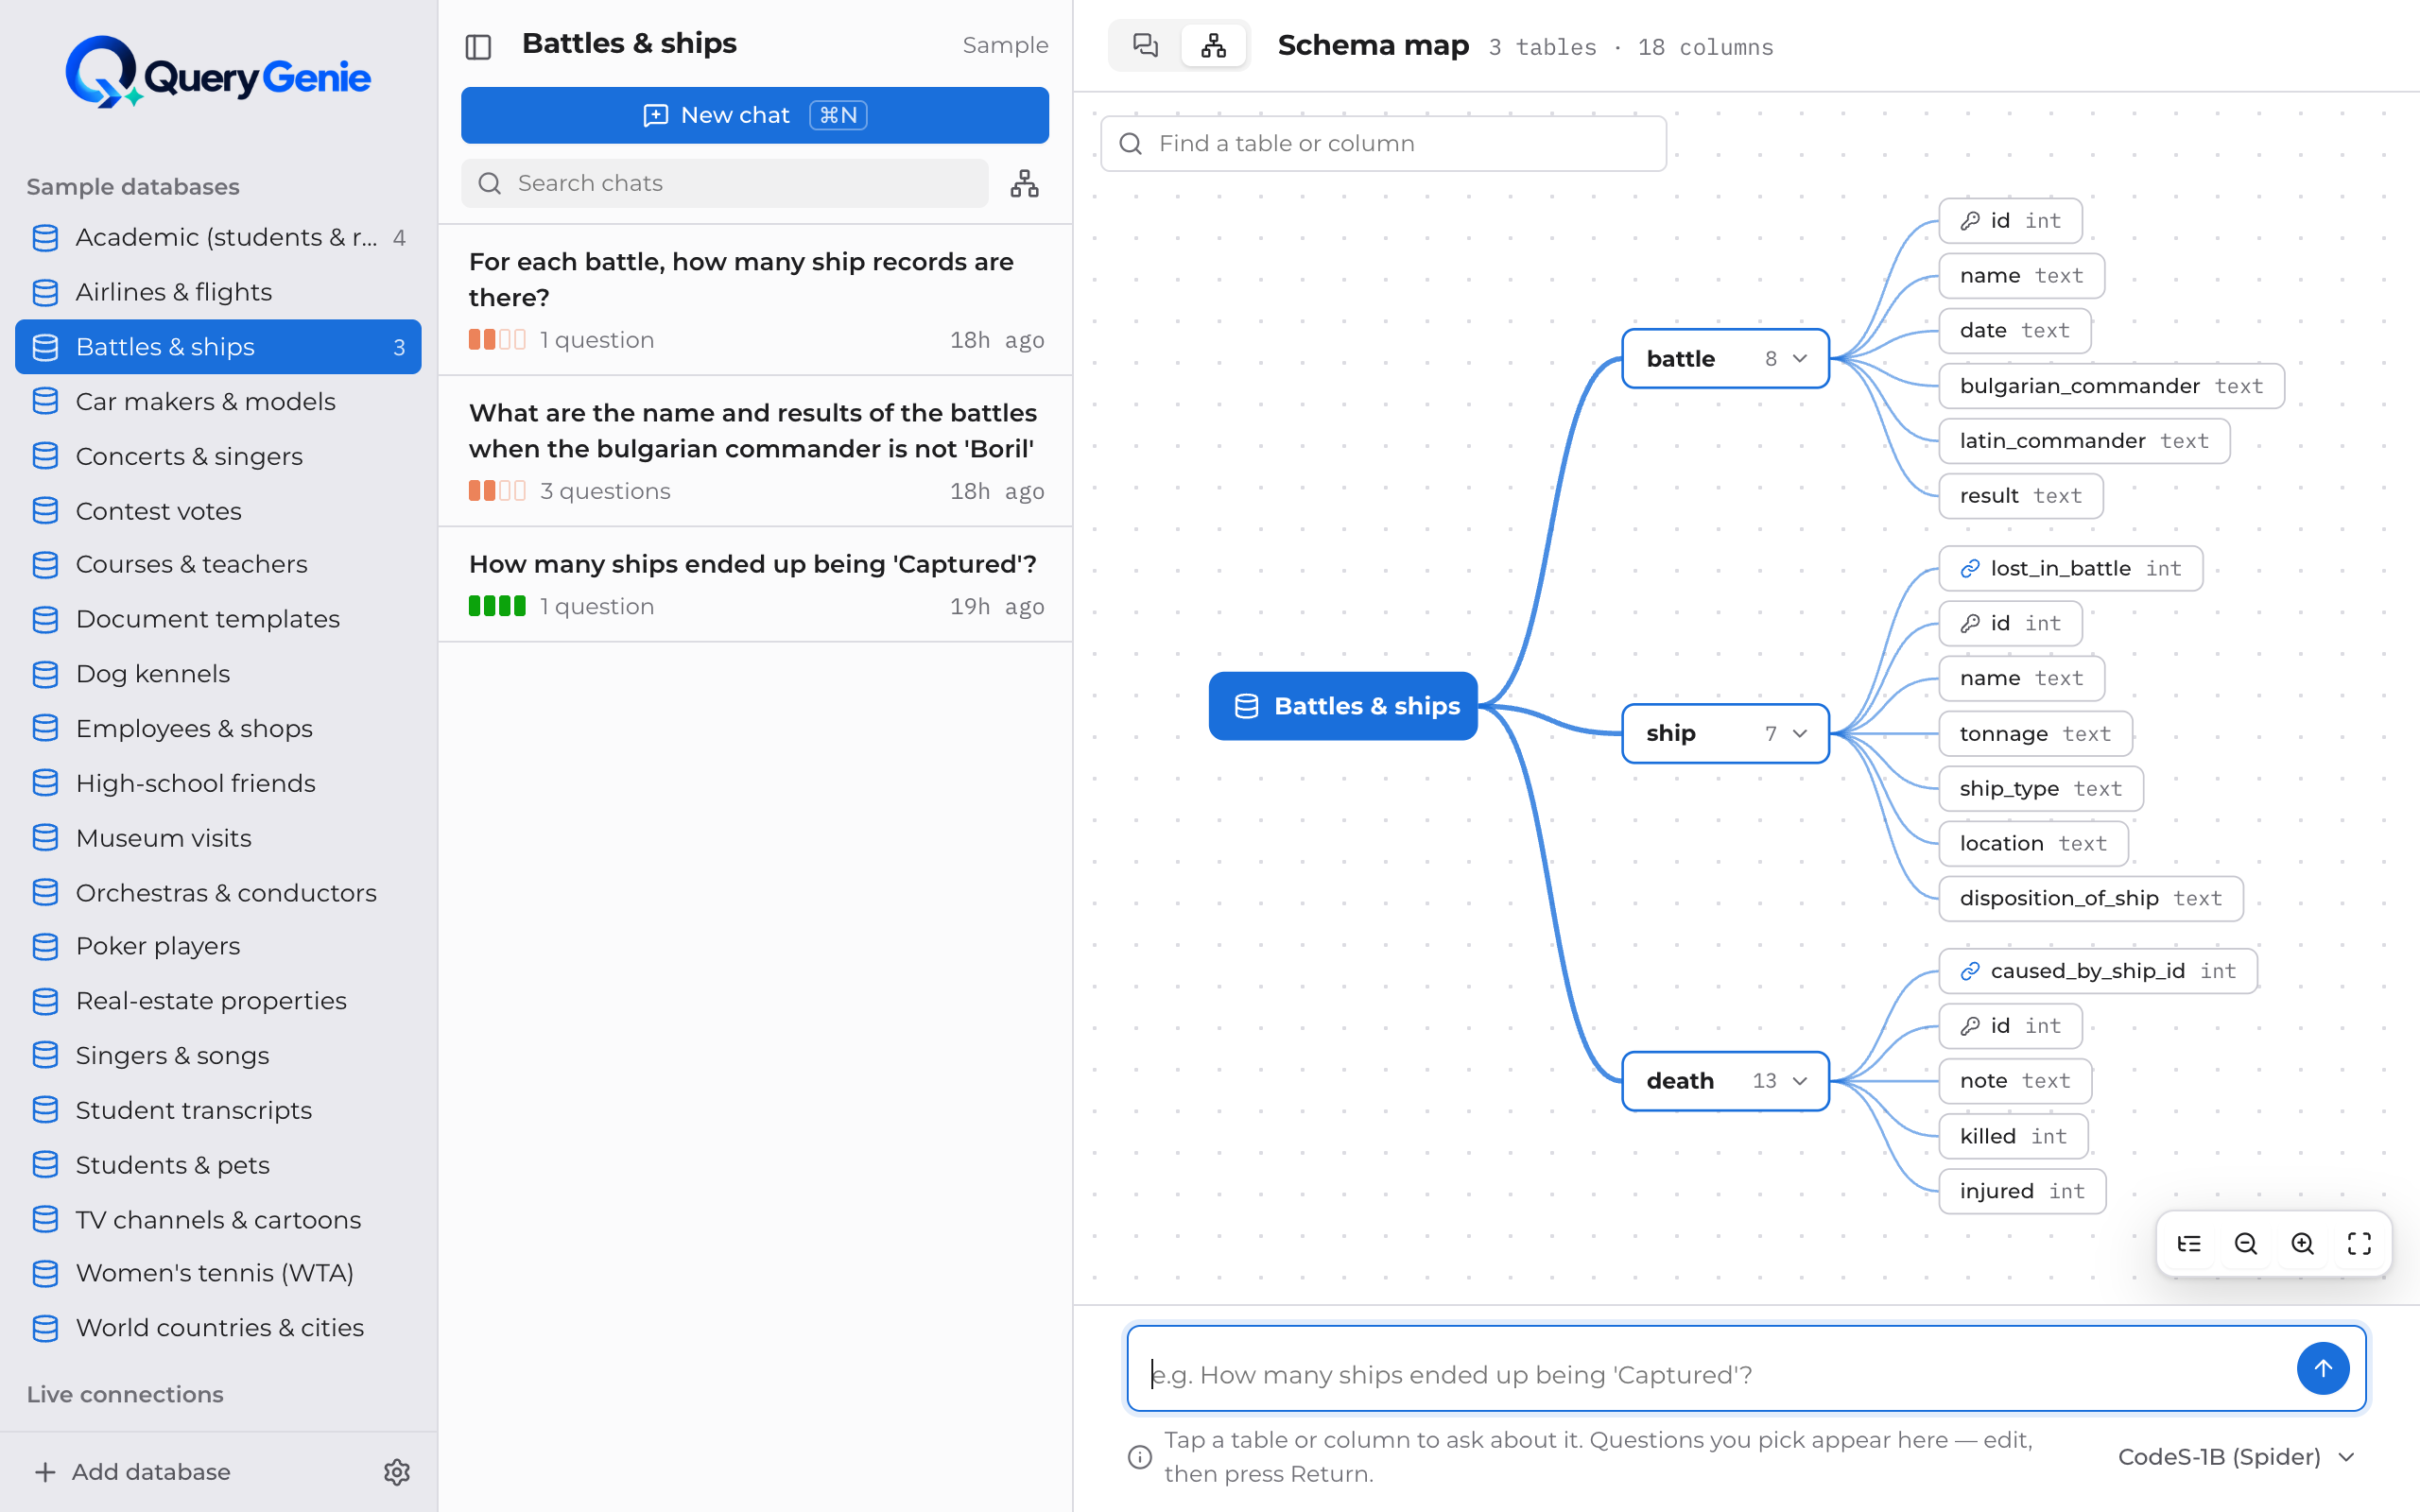
\includegraphics[width=\linewidth]{images/figures/app_schema_map.png}
	\caption{The schema map: tables, columns, primary keys and foreign keys of a Spider database.}
	\label{fig:app-map}
\end{figure}

\begin{figure}[!t]
	\centering
	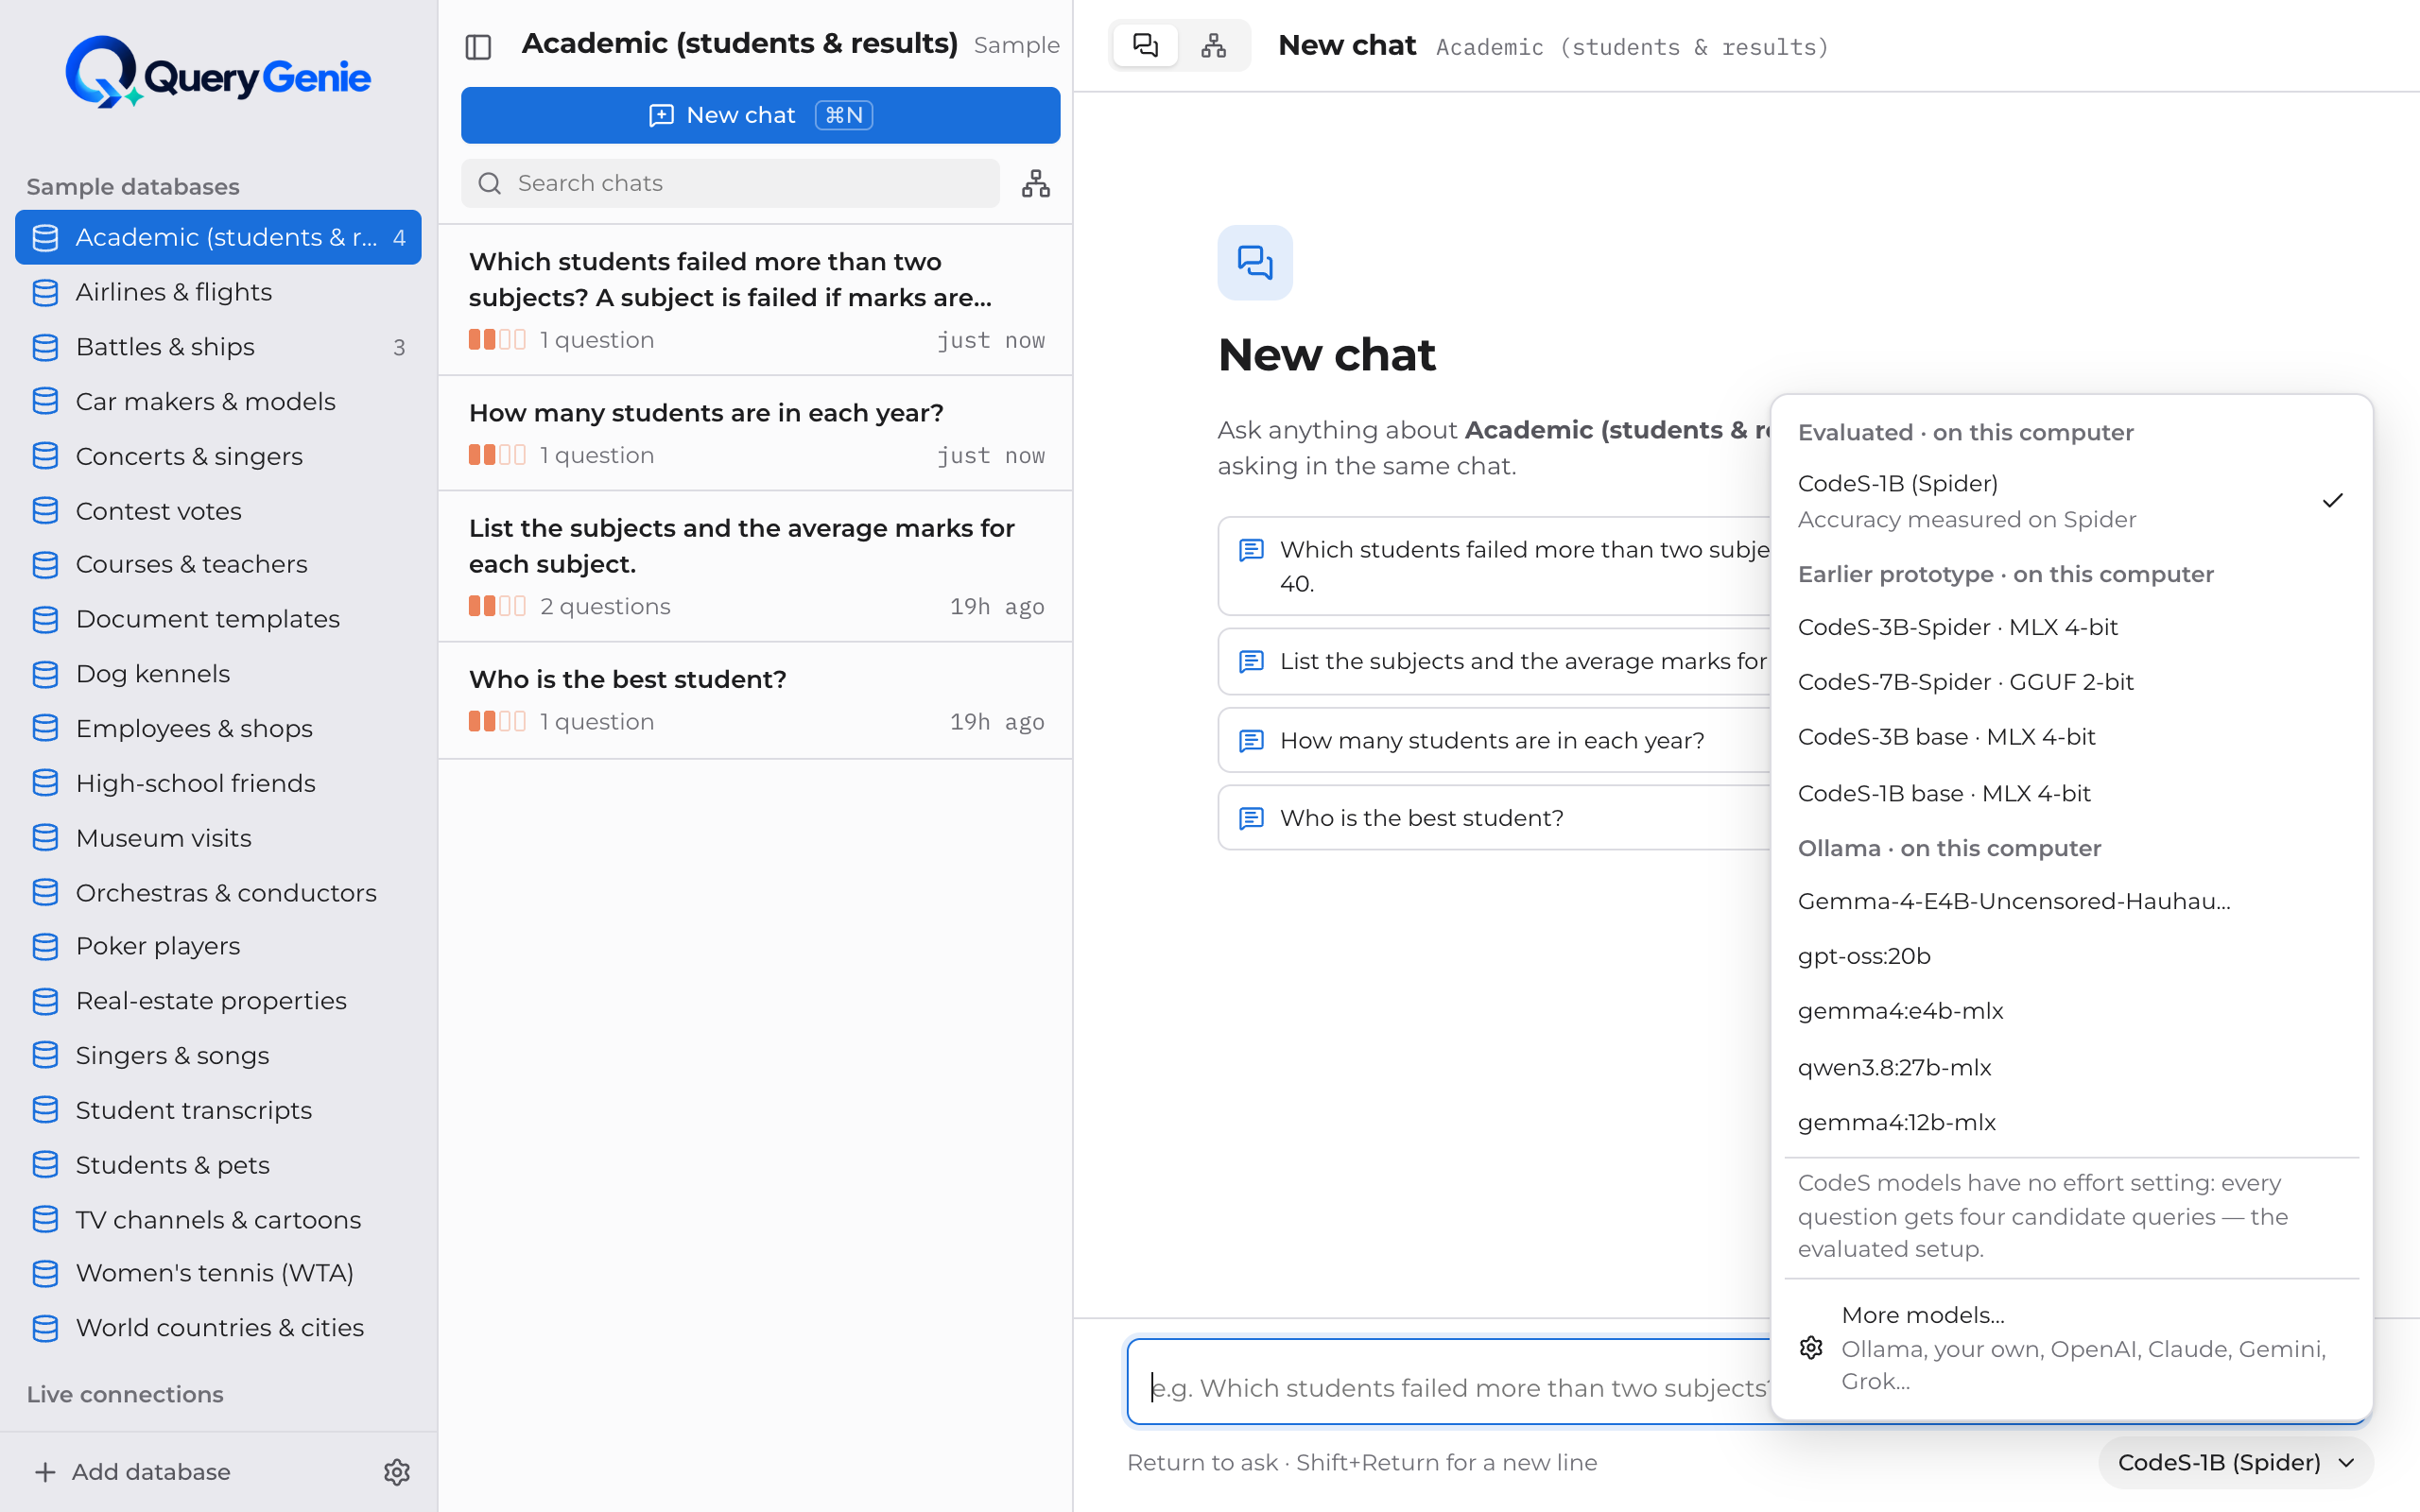
\includegraphics[width=\linewidth]{images/figures/app_model_picker.png}
	\caption{The model picker below the question box: the evaluated model, the earlier prototype's models and local Ollama models.}
	\label{fig:app-picker}
\end{figure}

A qualitative check on the bundled academic database shows both sides of the behaviour (illustrative, not a metric). With CodeS-1B the flagship question ``Which students failed more than two subjects?'' gets a wrong first answer, but the candidates split two against two, the answer is marked low confidence, the correct reading is offered as an alternative, and the strict setting abstains (Figure~\ref{fig:app-notsure}). A system that says when it is unsure is only as useful as that signal is honest, which is why the application shows its measured operating points rather than a single headline number.

\section{Differences from the authors' setup}

The reproduced accuracy is within 0.1 points of the paper, so the remaining deviations appear to have little effect on this benchmark. They are recorded in Table~\ref{tab:dev} for completeness.

\begin{table}[!t]
	\centering
	\caption{Remaining deviations from the authors' setup.}
	\label{tab:dev}
	\resizebox{\textwidth}{!}{%
	\begin{tabular}{|l|l|l|}
		\hline
		\textbf{Deviation} & \textbf{Cause} & \textbf{Observed or expected effect} \\ \hline
		Newer PyTorch and transformers & The pinned stack does not build on current Python & The authors note newer versions shift inference slightly; no measurable gap remains \\ \hline
		Distinct-value scan instead of Lucene BM25 & Avoids the Java / pyserini dependency & Superset of the authors' candidates; matched values may differ in number and order \\ \hline
		Schema item classifier not applied & Checkpoints on rate-limited Google Drive & Full schema passed; Spider databases are small \\ \hline
		Tesla T4 instead of A800 & Available hardware & Same precision (fp16) and batch size (1) as the authors' inference \\ \hline
		EX only; test-suite accuracy TBD & Test-suite databases not obtained & Test-suite accuracy (paper: 72.2\%) not yet reported \\ \hline
		Repository uses DeepSpeed ZeRO-2; paper states ZeRO-3 & Found while annotating the paper & Affects pre-training only, which was not reproduced \\ \hline
	\end{tabular}}
\end{table}

The largest lesson of the reproduction is about measurement rather than modelling. For a month our numbers sat 4 to 13 points below the paper, and the gap was blamed in turn on the prompt, the value retriever and the schema filter. The audit showed that about 4.4 points of it were our own scoring. Reproducing a result means reproducing the evaluation, not only the model.

\section{Source code and how to run it}

All code, results and documents are in the project repository on GitHub, \url{https://github.com/jayakanthh/QueryGenie}, with the supervisor added as a collaborator. The code is released under the Apache 2.0 licence. The repository is organised as follows:

\begin{itemize}
	\item \path{querygenie/} --- the evaluated core: the CodeS pipeline, the model wrapper, the abstention logic, the database catalogue and the connectors; the authors' utilities are included unmodified.
	\item \path{desktop/} --- the desktop application (native window, interface, first-run setup, packaging).
	\item \path{research/} --- the Colab evaluation harness, the abstention analysis, the dataset analysis of Chapter~3 and the notebooks.
	\item \path{results/} --- the run log, the harness audit, the ablation, abstention and comparison results, the figures, and the four-candidate record of run T2-006.
	\item \path{legacy/} --- the earlier web prototype, kept for the record; \path{tests/} --- model-free tests.
\end{itemize}

\textbf{Reproduce the results (GPU, about one hour).} Open \path{research/notebooks/02_tier2_colab_eval.ipynb} in Google Colab with a T4 runtime and run the Week-10 cell. It downloads Spider and the model from Hugging Face, evaluates all 1,034 questions with the official evaluator, and saves the predictions and the four-candidate record.

\textbf{Reproduce the enhancement analysis (CPU, seconds).}
\begin{lstlisting}[language=bash, caption={Significance tests, operating points and the accuracy--coverage figure}]
python research/abstention.py results/dump_T2-006.jsonl
\end{lstlisting}

\textbf{Run the application.}
\begin{lstlisting}[language=bash, caption=Running QueryGenie from source]
python3 -m venv .venv && source .venv/bin/activate
pip install -r requirements.txt
python desktop/main.py
\end{lstlisting}

\textbf{Tests (no model needed).} \texttt{python -m pytest tests/ -q}.
